\documentclass[titlepage,a4paper]{jsarticle}
% \documentclass[titlepage]{jarticle}
\usepackage[dvipdfmx]{graphicx}
\usepackage{listings}
\usepackage{here}
\usepackage{amsmath}
\usepackage[hyphens]{url} % 先にurlパッケージ読込
\usepackage[hidelinks,dvipdfmx]{hyperref}
%高専のstyファイルから拝借
% \RequirePackage{geometry,array}

% % \zw と \zh の定義
% \providecommand{\zw}{zw}
% \providecommand{\zh}{zh}

% \geometry{left=30mm,right=30mm,top=30mm,bottom=30mm}

\renewcommand{\baselinestretch}{1.25}
%
\lstset{
  basicstyle={\ttfamily},
  identifierstyle={\small},
  % commentstyle={\smallitshape},
  keywordstyle={\small\bfseries},
  ndkeywordstyle={\small},
  stringstyle={\small\ttfamily},
  frame={tb},
  breaklines=true,
  columns=[l]{fullflexible},
  numbers=left,
  xrightmargin=0zw,
  xleftmargin=3zw,
  numberstyle={\scriptsize},
  stepnumber=1,
  numbersep=1zw,
  lineskip=-0.5ex,
  language=java
}
\renewcommand{\lstlistingname}{ソースコード}
\makeatletter
\newcommand{\figcaption}[1]{\def\@captype{figure}\caption{#1}}
\newcommand{\tblcaption}[1]{\def\@captype{table}\caption{#1}}
\makeatother
\begin{document}
\title{測量技術の歴史について}
\author{情報・経営システム工学分野B3\\24336488 本間三暉}
\date{2024年6月26日}
\maketitle
\section{測量の起源と古代エジプトの発展}
測量の起源は紀元前3000年ごろのエジプトにまで遡る.

現在はアスワン・ハイ・ダムが建設されたことによって反乱することのないナイル川だが,
ダムが建設される以前は毎年夏になると季節風という海から陸に向かって湿った風が吹くことによる大量の降水によって必ず河川氾濫していた.
この氾濫により上流にあるエチオピア高原から肥沃な土壌が流れてきて,ほとんど雨が降らないエジプトの農耕と文明の発展を支えた.
このことは人々の生活にも大きな影響を与え,氾濫時期を知るためにシリウス暦が作られ,ナイル川の水位を知るための水位計が各地に設置された.
紀元前3000年ごろのエジプトでは氾濫のたびに区画が破壊されるため,そのたびに区画を作り直すための測量が行われ土地の配分が行われた.
このときに使われたのが,3:4:5の比率で印をつけた縄を張って畑の直角をとり,氾濫で流された農地の境界を復元していた.

ピラミッドの建設では測量技術が使用され,ピラミッドの平均辺長が230.36mに対してピラミッドの最長辺と最短辺の差が20.07cmしかないほど正確に建設されている.
また,ピラミッドの西北隅から東南隅に向かっての勾配は約1.27cmであり,ほぼ水平であることがわかっている.
四隅の直角についての誤差は最大で3.5’(分)であり,辺は真北を向いている.

紀元前2500年頃には水準測定器,垂直確定器,定規といった測量に必要な機器が既に使われていた.
古代エジプトで発達した測量技術はローマ,ギリシア,アラビアへと受け継がれ広まっていった.

\section{地図の始まり}
農耕や建設などの大規模な作業を行われるようになると,大勢の人々の協力が必要になった.
次第に指導者の下で多くの人々が働くようになり国家が成立すると,
人々が争わないように耕地の境界を定めたり,公平な課税を行うために,土地が測量され,地図に記録されるようになった.
これが地籍図の始まりである.
バビロニアでは粘土板,エジプトではパピルスという植物の葉を編んだもの,中国では絹に描かれていた.
紀元前2000年ごろになるとバビロニアや中国で全ての知識を一望に表そうとして世界図が作られた.
世界と言っても地球全体ではなく,彼らの知りうるすべての土地という意味である.

バビロニアに現存する世界最古の粘土板の世界図は紀元前700年ころのものと推定されている.
バビロニアの粘土板で作られた地図を図\ref{map}に示す.
\begin{figure}[t]
      \centering
      \begin{minipage}[]{0.45\hsize}
            \centering
            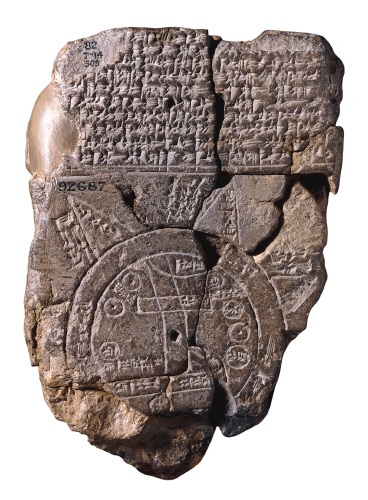
\includegraphics[width=4cm]{img/babironia.jpg}
            \caption{バビロニアの世界図(地図の歴史 / 古代より引用)}
            \label{map}
      \end{minipage}
      \begin{minipage}[]{0.45\hsize}
            \centering
            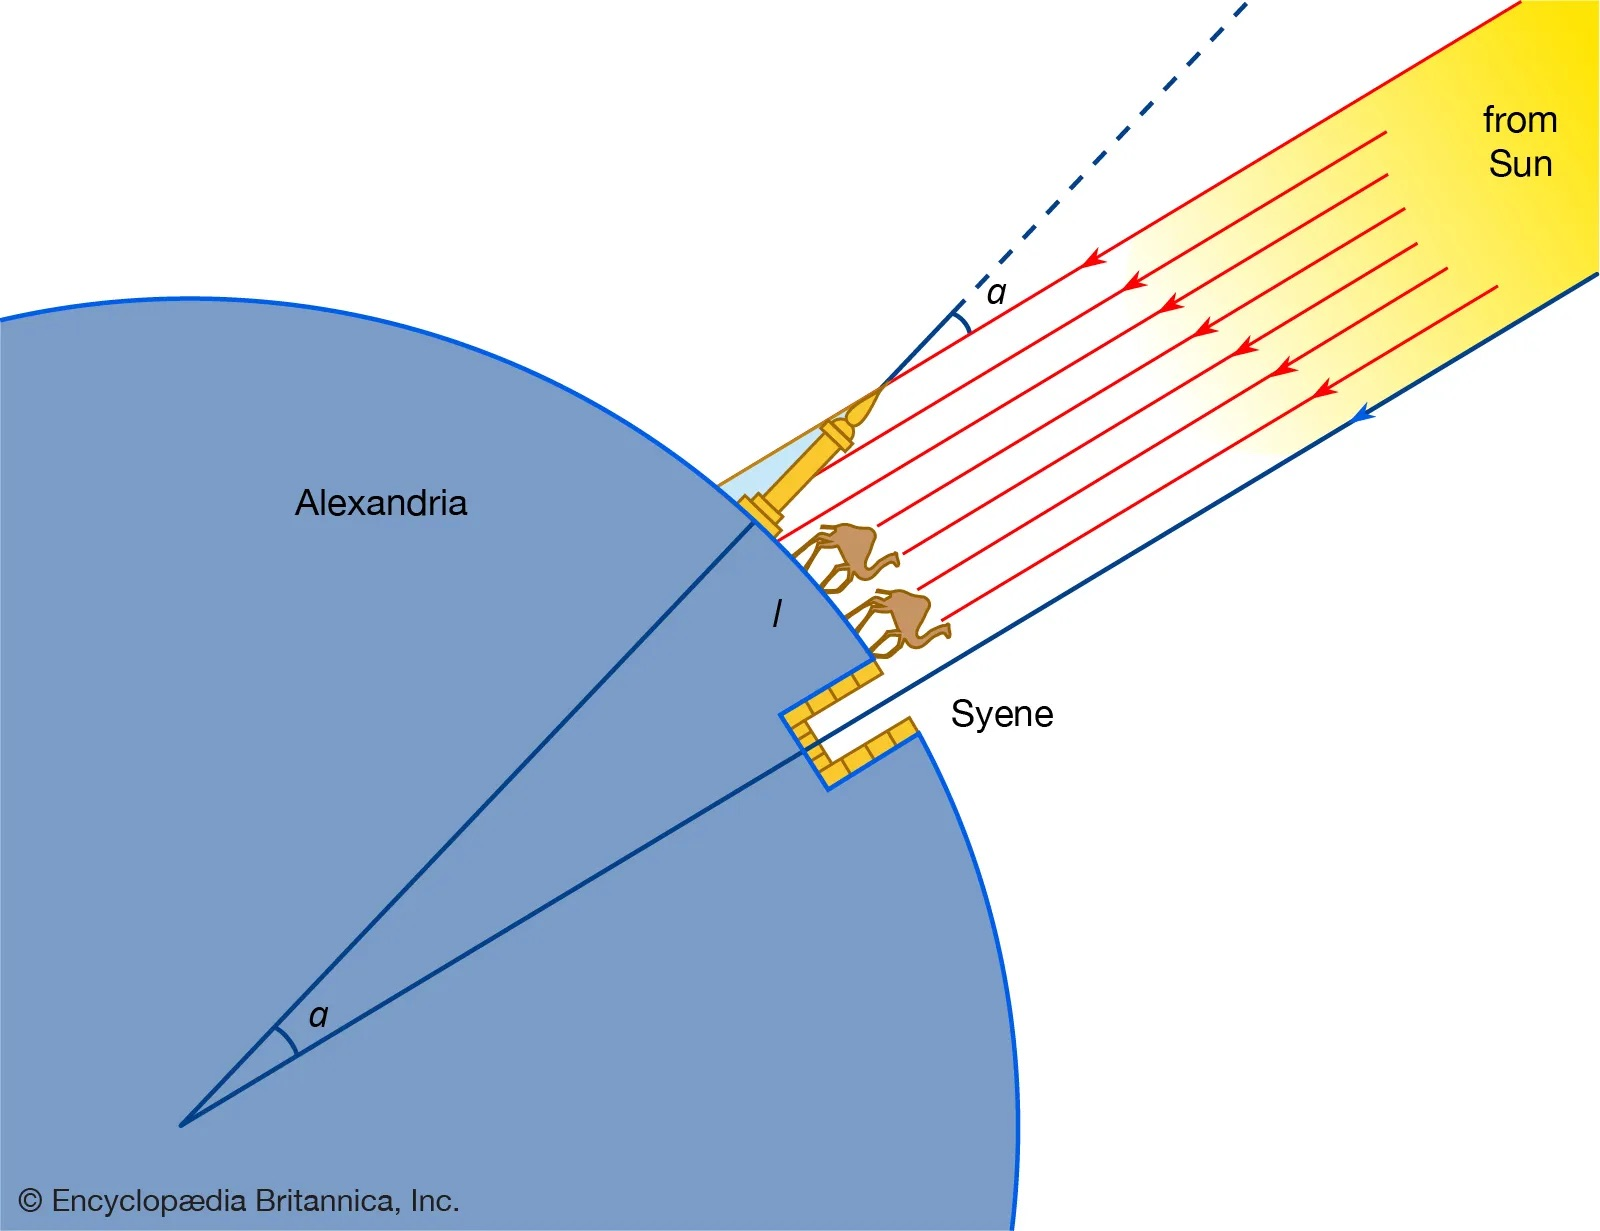
\includegraphics[width=5cm]{img/hidokei.jpeg}
            \caption{太陽の角度から地球の大きさを求める}
            \label{hidokeii}
      \end{minipage}
\end{figure}
円と直線を組み合わせた単純なものであるが,首都バビロンを中心とする円形の陸地が海に取り囲まれている.
小アジア(トルコのアジア側)の山岳地からペルシア湾までが含まれていて,ユーフラテス川も描かれている.

\section{大地は球である}
4大文明(メソポタミア,エジプト,インダス,黄河)のころに作られた世界図を見ると,彼らはまだ大地が平面であると考えていたようである.
一方で,天体を観測して暦を作ることは世界各地で行われるようになり,繰り返されるリズムの中から自然にはルールがあることは理解され始めていた.
ギリシアでも初期の世界観はバビロニアの影響を受け,大地は平らな円盤であると考えられていた.
地理学者のへカタイオス(550?B.C.~475?B.C.)が作成した世界図は,\textbf{全世界の地形とともに海洋と河川のすべてを彫り込んである銅板}と伝えられ,
地中海の海岸線はかなり正確に描かれていた.
しかし大地の形は平らな円盤で,周囲は\textbf{オケアノス}と呼ばれる架空の大洋に囲まれていると考えていた.

ピタゴラス(570?B.C.~497?B.C.)やアリストテレス(384B.C.~322B.C)などの天文学や幾何学を学んだ科学者が大地について考察を始めた時,
大地の形が平らな円盤だと考えられてきた世界観は一変する.
彼らによって太陽や月が球体であること,南北に長い距離を移動すると星の高さが変化すること,
月食のときに月面に映る地球の影は円または円弧であること,沖合いの船はマストだけが見えることなどの根拠から大地が平らではなく球であるという説が唱えられた.

\section{日時計による地球の大きさの計測}
地中海に面したエジプトの港町であるアレクサンドリアの図書館長であったエラトステネス(276?B.C.~196?B.C.)は,
同じ経度上にある2地点間で,距離と同時刻の太陽の高度を計測することで地球の大きさを計算できる図\ref{hidokeii}のような方法を思いついた.
エラストテネスは\textbf{ナイル川上流のシエネでは夏至(北半球で昼が一番長い日,6月22日頃)の日に井戸の底まで太陽が差し込む井戸}があることを知り,
あとはアレクサンドリアでの太陽高度と,アレクサンドリアからシエネまでの距離を調べるだけであった.
太陽高度は日時計として使われているオベリスクと呼ばれる石の塔が作る影を測り,距離の測定方法は記録に残っておらず,歩測で求めたと推測される.
これらの情報から計算した結果およそ44,500kmと求められ,実際の値より1割増であるという結果が得られた.

当時,まだ地中海の外の世界についてはほとんど分かっていなかったが,地球の大きさを計算によって求めることができていた.
この幾何学を応用した地球の円周の大きさの計算こそが測地学の基礎である.

\section{日本の測量史}
3世紀後半には近畿・瀬戸内海沿岸・九州北部には墳墓や陵墓が築造されはじめましたが,大規模な古墳の残存状態から,構築の過程で方位や距離・寸法など精密な測量が行われたことがうかがわれる.
5世紀になると大陸から多くの人々が渡来し,大陸の技術が導入され始めた.

607年,小野妹子を始めとする遣隋使を派遣し中国の制度や文化を導入した.その時に測量技術が日本に伝わった.
その後\textbf{班田収授法}という,政府から受田資格を得た遺族や人民へ農地が支給され,その際に全国の農地が測量されたとされる.
そこで長さや広さといった単位も制定された.

\section{日本の測量士}
日本で始めて測量士になったのは,伊能忠敬である.
江戸時代の商人でもあった彼は,17年の歳月をかけて日本全国を測量し,\textbf{大日本沿岸輿地全図}を完成させた.
伊能忠敬は基本的に自分の歩幅を測り,歩いて距離を測った歩測という手段で測量を行った.
また,歩測以外にも現代の\textbf{水平器}や\textbf{勾配計}のような機能を持った道具を用いていたとされる.

\section{コンパスの誕生}
11世紀末の中国では,水に浮かべた磁針が北を指すことが知られていた.
海のシルクロードという元帝国によって整備された海上交易路を通り,インドアラビアを通り,13世紀には海運国イタリアに達し,
水の代わりに方位盤に立てた軸に磁針を乗せる工夫がされて,航海用羅針盤が発明された.

コンパスで港からの進行方向を確認し,浮きの付いたロープで距離を確認して地図上に航路を記し,海岸の形状をスケッチを行っていた.
コンパスの登場により,初めて測量に基づいた地図が作られるようになった.

その後,マルコ・ポーロの東宝見聞録などアジアの情報が入ってくると,地図にも反映され始めた.
それと同時に,進んだイスラム文化やアジア文化に衝撃をうけ,世界に関心を持つようになっていった.
その後,コンパス・機械時計・緯度測定器といった測量技術の進化や安定した大型の帆船などにより,外洋に乗り出す大航海時代となっていく.
\section*{参考文献}
\begin{enumerate}
      \item 【測量技術の歴史】測量は紀元前3000年のエジプトから存在していた | 東京法経学院 資格コラム\\
            \url{https://www.thg.co.jp/douyo/shikaku/sokuryoshiho/surveying-technique-history/}
      \item モンスーンの意味や定義 わかりやすく解説 Weblio辞書\\
            \url{https://www.weblio.jp/content/モンスーン}
      \item 測量年表\\
            \url{https://www.jsurvey.jp/soknohi/sok-nenpyou.htm}
      \item 測量の歴史 | 大誠色々\\
            \url{http://www.taiseiks.jp/blog_contents_012.html}
      \item 日本の測量史 目次\\
            \url{http://uenishi.on.coocan.jp/}
      \item 地図の歴史\\
            \url{https://atlas.cdx.jp/history/history.htm}
      \item Eratosthenes | Biography, Discoveries, Sieve, \& Facts | Britannica\\
            \url{https://www.britannica.com/biography/Eratosthenes}
      \item 日本の測量の歴史 | 長期休暇中の営業日程や測定会社を選ぶコツなどのコラムを発信 | 大阪で建設や管理を補佐する株式会社セキ測量調査\\
            \url{https://seki-si.co.jp/blog/detail/20210406131433/}
\end{enumerate}
% 
\end{document}